% !TEX root = ../main.tex
%==========================================%

\section{Introduction}\label{Intro}

\textblue{Give a brief introduction on Bitcoin and crypto-currencies and the state of stablecoins in general.}


% It is difficult to define a stable coin because, the more we read, it captures a negative sentiment (what a coin ought not to be) more than what a coin ought to be. It ought not to be like Bitcoin, whose volatility is high.

% Stablecoins are a topic of recent interest. A lot of blogs and some academic articles have systemized them. We know that the reader of this paper is expecting a chart of coins and what mechanisms they use: we do provide that, but we do not consider that the core contribution of the paper at all. Instead we really dug into finance to deeply understand the core methods and mechanisms that are employed for reducing volatility of a coin. We feel our paper is closer to a tutorial on stablecoins where we try to eliminate all the jargon (which is often misused and imprecisely applied) to explain the concepts, as well as drawing out appropriate foundations from finance.

% Example: if we described the approach of stable coin in two simple words: ``currency board'' and you need no further explanation (just, perhaps, some details on the parameters), this paper is not for you. If you have heard the term and have a vague sense of how it works, but couldn't really explain it or why it achieves stability, this paper is for you. If you have never heard the term, this paper is also for you.

% Two basic concepts: (1) a tokenization of a fiat currency (say a digital dollar) or any asset or asset portfolio of assets. This is an old idea: liberty reserve, eGold. (2) a low-volatility coin that is tied to any existing asset. For example, with USD as the baseline, Euros are much more stable than Bitcoin. It is not because Euros are backed by USD or have any direct reference to the USD. It is because USD and Euros use the same model, a central bank management, with similar inputs (the interest rates their customers, commercial banks, use when lending cash to each other to meet various legal requirements that help ensure the banks will have enough cash on hand to server their customers and can withstand some of their investments going bad without going bankrupt).

% Most of the coins are mostly focusing on the supporting infrastructure, maybe we also have to talk about the supporting infrastructure of the stablecoin
% Talk about the crypto custodianship somewhere in the paper
%==========================================%

\subsection{Motivation} %need a better name
\textblue{In this section we talk about volatility and what does stability mean, and we make argument that we're not economist and everything is explained in our own language}
Cryptocurrencies have gained a wide application after Bitcoin was first introduced in Satoshi Nakamoto’s (pseudonymous) 2008 whitepaper~\cite{nakamoto2008bitcoin}. For Bitcoin and any other cyptocurrency to function as money, they need to fulfill a set of properties that determine the strength and adoption of them \ie they are expected to serve as a medium of exchange, a unit of account, and a store of value. However, due to high fluctuations in their prices, majority of the cryptocurrencies do not meet these properties and hence they cannot be adopted as money~\cite{overview}.

Having said that, the volatile nature of cryptocurrencies (\eg Ether, Bitcoin) has raised the interest into what is known as stablecoin. Stablecoins (\ie cryptocurrencies with stable price) ensure that the fluctuation in the value remains low. Figure~\ref{fig:btcandfiat} illustrates the volatility of Bitcoin's value, when compared to fiat currencies, and the change of values of EUR, GBP, CAD, and BTC with respect to USD over time. Monthly values between January 2016 and November 2018 are shown. According the figures, while fiat currencies show stable behaviour, Bitcoin's value changes drastically over time, which makes it a non-stable cryptocurrency.

%========================%
\begin{figure}[!htb]
	\centering
	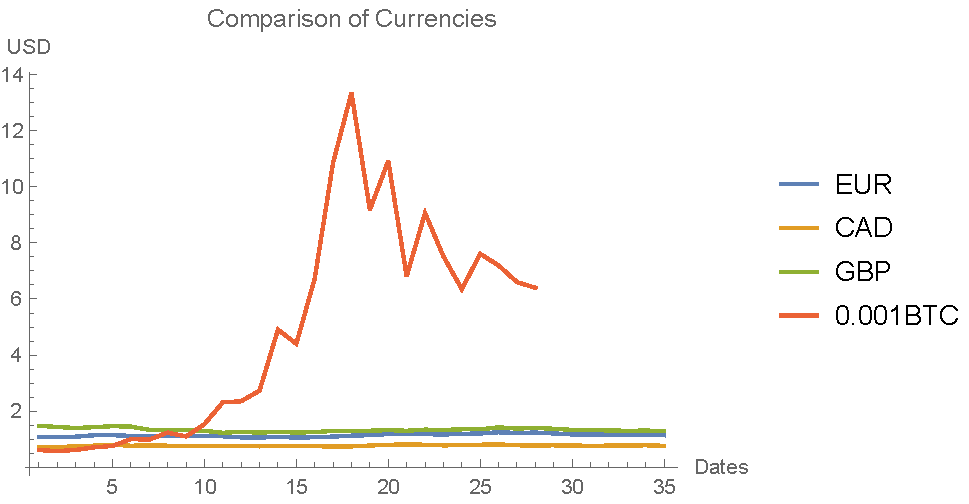
\includegraphics[width=0.75\textwidth]{figures/graph1.pdf}
	\caption{\label{fig:btcandfiat}Comparison among fiat currencies and Bitcoin: The values are retrieved on the first day of each month. A fraction of Bitcoin (1/1000 BTC) is plotted.}
\end{figure}
%========================%

Figure~\ref{fig:btc} shows the change of value of Bitcoin with respect to USD and gold. The value changes happen in directions 2 and 6 (Figure~\ref{fig:legend}). The part of plot in direction 2 means that Bitcoin is gaining value against gold and USD. This can also be interpreted as both gold and USD are losing value relative to Bitcoin. %However, the first explanation is more likely to be the case, as only Bitcoin's value is changing compared to two values (USD and gold) changing.
Also, the fact that the plot is located on the diagonal shows that Bitcoin gains/loses value against both USD and Gold at the same time. This indicates that the changes in the values of USD and gold are highly correlated.

Considering these facts, there is a desire to design stablecoins with the stable nature of the fiat currencies together with the decentralized nature of the blockchain which is the underlying technology of cryptocurrencies.

%==========================================%

\section{Preliminaries}

\subsection{Valuation}
% Every thing has two prices

How do we assign value to something? how do we establish what something is worth?
The value is usually given in some units of account (\eg CAD). When we establish a value for something, we do. not really claim what the value and what it worths, instead, we establish a value of its exchange. For example, today Alice is willing to pay 500 CAD for Bob's phone, whereas tomorrow, she will pay 600 CAD. What happened in this case? It could be (i) the value of money (CAD) going down or (ii) the value of good (phone) going up. Thus, in order to establish how much value something has, we should think of it in terms of being an exchange rate (the exchange rate between that asset and some other valuable assets). In other words, if Bob is willing to offer his phone for 1000 CAD, does it mean that it worths 1000 CAD? What we know about is that the value of Bob's phone is somewhere between 500 CAD (which Alice is willing to bid) and 1000 CAD (which Bob is willing to accept/ask). Therefore, the value of an object is not a single number and we can think of it as an interval between a least amount somebody wishes to sell for and the most amount somebody wishes to pay for that object, this interval is called bid-ask. If an ask comes below a bid, then the transaction happens and that amount is recorded as the final price, we call this \textit{crossing}. \par
What actually happens when they cross? Assume that they cross in such that Bob wants to pay (bid) 600 CAD for Alice's phone while Alice wants to sell (ask) it for 500 CAD. What happens in the real world is (i) either one party goes first and advertises a bid or an ask and when it crosses with other party's complimentary bid or ask, she accepts it. (ii) both parties advertise and they do not know about each other's price, so when they cross, the market decides (usually they pick the midpoint between the two). \par
When there is a cross, you have a price that is used for selling the object, that price is a last transaction price. So three values are actually important: 1) What is the most somebody is willing to pay for the object, 2) What's the least somebody is willing to accept for it, and 3) what was the last price this object is sold out. The value we see in the newspaper is always the last price, although it does not represent how much the object worths. In fact, we cannot actually say that and the best way to say that is when the bid-ask interval is really small. Assume that the interval is only 1 cent difference, in this case we can make sure what is the value and we are sure down to a cent. When the market changes so fast, the last price gives a lot of information on how much something worths, however, the last price that belongs to 30 years ago does not reveal a lot of information.

\subsection{Exchange}

\clearpage
\subsection{No-Seignorage Theory of Money}

To explain Bitcoin's exchange rate with fiat currencies, an oft-repeated theory has emerged that attributes Bitcoin's value to the hydro consumed by blockchain mining. While imprecise, the theory suggests that if a valuable resource $x$ is consumed to produce $y$, the value of $x$ is imparted into $y$. Setting aside the nuance that the hydro contributed to the Bitcoin system only indirectly produces new coins (it produces blocks, and blocks produce coins only for now), there is no economic principle underlying this transfer of value.

If Alice goes to Peter Luger's in Brooklyn, consumes a \$100 ribeye, and mints a literal shitcoin out of the result --- is that coin worth \$100 because it is ``backed'' by \$100 worth of steak?

%==========================================%

\section{Systemization of stablecoins and Justification}
\textblue{The main meat of the paper where we place the table and explain it.} \par

% Dollar tokenization vs. low volatitility

% !TEX root = ../main.tex


%-------------------Fancy Table ----------------------%

% = = = Rotated Table Entry \headrow


\newcommand{\headrow}[1]{\multicolumn{1}{c}{\adjustbox{angle=65,lap=\width-0.5em}{#1}}}

% = = = Table bullets: \full and \prt (full and part)

\newcommand{\full}{$\bullet$}
\newcommand{\prt}{$\circ$}
% ------------------------------------------------------------------------------------------------------------------------------------------------%
%Stablecoin projects%

\definecolor{UnitedNationBlue}{rgb}{0.30,0.53,1}
\definecolor{LightSteelBlue}{rgb}{0.69,0.77,0.87}
\definecolor{LightGrey}{rgb}{0.83,0.83,0.83}


\begin{table*}[t]
\centering

\begin{tabular}{|l|l|l|l|l|}

\hline
\rowcolor{lightgray}
\textbf{Class} & \textbf{Mechanism} & \textbf{Resembles} & Rank \\  \hline
% = = = = = = = = = = = = = = = = = = = = = = = = = = = = = = = = = = = = = = = = = = = = = = = = = = = = = = = = = = = = = = = = = = = = = = %
\multirow{17}{*}{Backed}		
						& \multirow{8}{*}{Directly-Backed \& Redeemable$^{\dagger}$}	& USDC 			& 20 \\ \cline{3-4}
						&													& TrueUSD 		& 26 \\ \cline{3-4}	
						&													& Paxos 			& 38 \\ \cline{3-4}		
						&													& Gemini Dollar 	& 52 \\ \cline{3-4}
						&													& StableUSD (USDS) & 685 \\ \cline{3-4}
						&													& Stronghold USD 	& 891 \\ \cline{3-4}
						&													& Petro 			& 1210 \\ \cline{3-4}
						&	& \multicolumn{1}{p{5cm}|}{Ekon, WBTC, emparta} & $\perp$ \\ \cline{2-4}
% = = = = = = = = = = = = = = = = = = = = = = = = = = = = = = = = = = = = = = = = = = = = = = = = = = = = = = = = = = = = = = = = = = = = = = %
						& \multirow{6}{*}{Directly-Backed}  							& Tether 			& 6 \\ \cline{3-4}
						&													& EURSToken 		& 95 \\ \cline{3-4}
						&													& BitCNY 			& 304 \\ \cline{3-4}
						&													& Terracoin 		& 1280 \\ \cline{3-4}
						&													& Saga 			& 1495 \\  \cline{3-4}
						&	& \multicolumn{1}{p{5cm}|}{GJY, Novatti AUD, UPUSD} & $\perp$ \\ \cline{2-4} 						
% = = = = = = = = = = = = = = = = = = = = = = = = = = = = = = = = = = = = = = = = = = = = = = = = = = = = = = = = = = = = = = = = = = = = = = %
						& \multirow{3}{*}{Indirectly-Backed}							& Dai 			& 57 \\ \cline{3-4}
                                                &													& BitUSD 			& 398 \\  \cline{3-4}
                                                & 													& Nomin			& $\perp$ \\ \cline{1-4}
% = = = = = = = = = = = = = = = = = = = = = = = = = = = = = = = = = = = = = = = = = = = = = = = = = = = = = = = = = = = = = = = = = = = = = = %
%						& \multirow{1}{*}{Market Manipulation} 						& NuBits			& 892 \\ \cline{1-4}
\multirow{5}{*}{Intervention}                                                           

% = = = = = = = = = = = = = = = = = = = = = = = = = = = = = = = = = = = = = = = = = = = = = = = = = = = = = = = = = = = = = = = = = = = = = = %
						& \multirow{2}{*}{Money Supply Adjustments}  				& Ampleforth		& $\perp$  \\ \cline{3-4}
						&   													& RSCoin 			& $\perp$  \\ \cline{2-4}
% = = = = = = = = = = = = = = = = = = = = = = = = = = = = = = = = = = = = = = = = = = = = = = = = = = = = = = = = = = = = = = = = = = = = = = %
						& \multirow{2}{*}{Asset Transfer}  							& NuBits			& 892 \\ \cline{3-4}
						&													& CarbonUSD		& 1262 \\ \cline{3-4}
						&													& Basecoin 		& $\perp$ \\ \cline{1-4}
% = = = = = = = = = = = = = = = = = = = = = = = = = = = = = = = = = = = = = = = = = = = = = = = = = = = = = = = = = = = = = = = = = = = = = = %
%						& \multirow{2}{*}{TBD: Internal }  								& Nautiluscoin 		& $\perp$ \\ \cline{3-4}
% = = = = = = = = = = = = = = = = = = = = = = = = = = = = = = = = = = = = = = = = = = = = = = = = = = = = = = = = = = = = = = = = = = = = = = %
\hline
\end{tabular}
\caption{Stablecoin proposals as of January 11, 2019. $\dagger$ \textit{Disclaimer:} Projects are classified according to what they assert; \eg we provide no warranty that projects classified as `redeemable' provide actual redemption of the assets that back their coins. Rank corresponds to \textit{CoinMarketCap}.\label{tab:stablecoins}}
\end{table*}
% ------------------------------------------------------------------------------------------------------------------------------------------------%





% Jeremy: How do we make a stable coin.
% Jeremy: Table here

\subsection{Redeemable and Directly-Backed.}
% Description of how it works: Desposit in bank, etc
% Justification that bids will never exceed $1: an arbitrageur will pay $1 to mint 1 XSC and the 1 XSC for the bid
% Justification that offers will be less than $1: an arbitrageur will purchase the 1 XSC and redeem it for $1
% Risk: not redeemable -> redemption is not 100%, the coin will be offered at less than $1. E.g., offers of $0.50, says 50% it can't be redeemed.
% Examples: Gemini


\subsection{Non-Redeemable and Directly-Backed.}
% Description of how it works. Deposit in bank, etc
% Justification that bids will never exceed $1:
% Justification that offers will be less than $1
% Examples: Tether
% Remarks:


\subsection{Non-Redeemable and indirectly-Backed.}
% Description of how it works.
% Justification that bids will never exceed $1
% Justification that offers will be less than $1
% Examples:
% Remarks: Oracles


\subsection{Redeemable and indirectly-Backed.}
% Description of how it works.
% Justification that bids will never exceed $1
% Justification that offers will be less than $1
% Examples:

 \subsection{Currency Board.}
% Description of how it works.
% Justification that bids will never exceed $1
% Justification that offers will be less than $1
% Examples:

\subsection{Algorithmic}

% Control system: input (metrics), make a decision, implement the intervention
% We cannot prove that something here works or not. It is all heuristics. We know this because central banks themselves operate on heuristics that change every couple of decades. Even if we cannot say something does work, we can point out a few suggestions that it will not work. Game-able inputs, inputs/interventions that have not worked for currency.

\subsection{Algorithmic with subjective external information}
% Description of how it works.
% Justification that bids will never exceed $1
% Justification that offers will be less than $1
% Examples: RSCoin

\subsection{Algorithmic with objective external information}
% Description of how it works.
% Justification that bids will never exceed $1
% Justification that offers will be less than $1
% Examples:

\subsection{Algorithmic with only internal information}
% Description of how it works.
% Justification that bids will never exceed $1
% Justification that offers will be less than $1
% Examples:

We performed a search query on \texttt{coindesk.com} and found the following projects which are mostly used in every articles published about stablecoins until January 11, 2019. \footnote{https://www.coindesk.com/} Table~\ref{tab:stablecoins} represents these projects and the methods they apply to achieve stability. (we should mention the search term that we used to extract our resources from coindesk)


\textbf{Distribution of articles speaking about stablecoin:} 2014: 2, 2017: 4, 2018: 112, 2019 (up to Jan 11): 4.


%==========================================%

\section{Investigation of gas volatility}
\textblue{in this section we have  a discussion about Gas: Gas is not a currency so you cannot buy things with it BUT you can have a smart contract and swap it with other tokens.  Gas is actually stable with respect to others, the reason ir's not obvious is human error and usability stuff. Gas is not pegged to anything. Also it would be nice to have a chart : Ether, Electricity (Global energy index), and Gas} \par
Our analysis in Section~\ref{Intro} shows that cryptocurrencies exhibit less stable behavior compared to fiat currencies. Hence, we aim to analyze the price stability of \emph{Gas}. In Ethereum blockchain, every transaction contains a number of operations and there is a precise amount of gas unit associated with each.\footnote{http://ethdocs.org/en/latest/contracts-and-transactions/account-types-gas-and-transactions.html\#what-is-gas} Since Ether is volatile, this concept is introduced to have fixed cost for operations. Thus, even though the price of Ether changes, the amount of Ether corresponding to a unit of gas decreases; so that users pay the same price for the transactions on the Ethereum blockchain. Hence, the notion of gas is yet to be investigated to find out whether it exhibits behavior similar to fiat currencies or cryptocurrencies.

%========================%

%\begin{figure}[!htb]
%	\centering
%	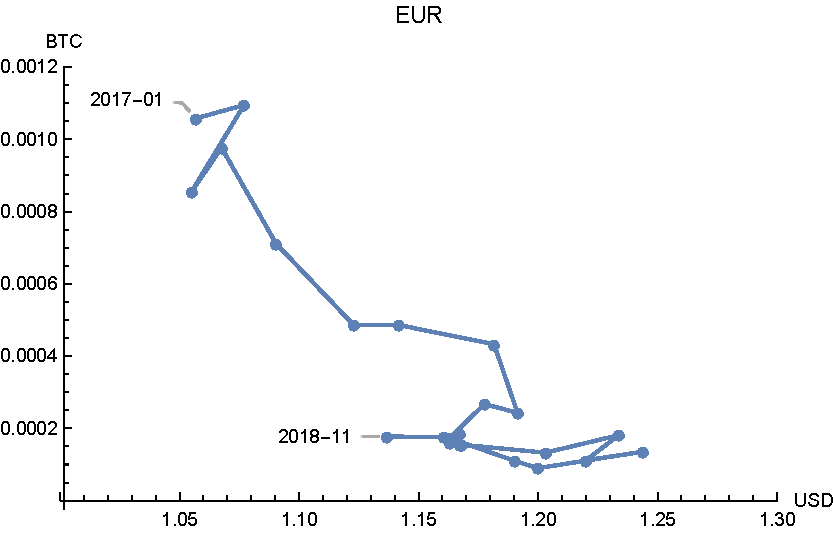
\includegraphics[width=0.95\textwidth]{figures/eur.pdf}
%	\caption{\label{fig:eur} EUR with respect to BTC and gold.}
%\end{figure}
%========================%

%\begin{figure}[!htb]
%	\centering
%	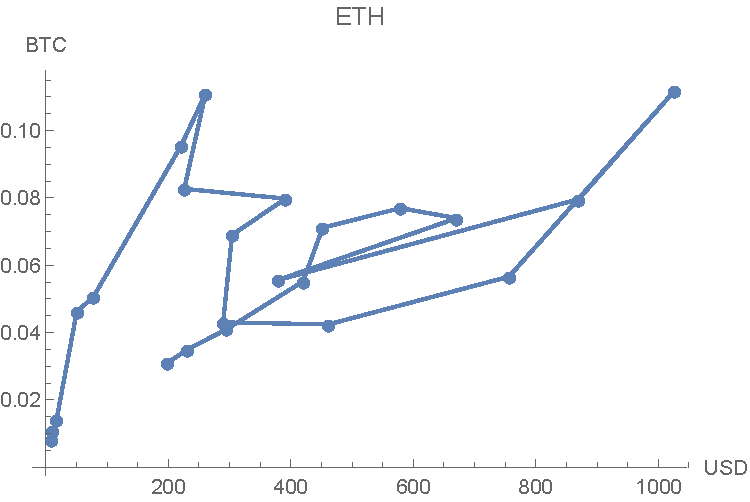
\includegraphics[width=0.95\textwidth]{figures/eth.pdf}
%	\caption{\label{fig:eth} ETH with respect to BTC and gold.}
%\end{figure}
%========================%

%\begin{figure}[!htb]
%	\centering
%	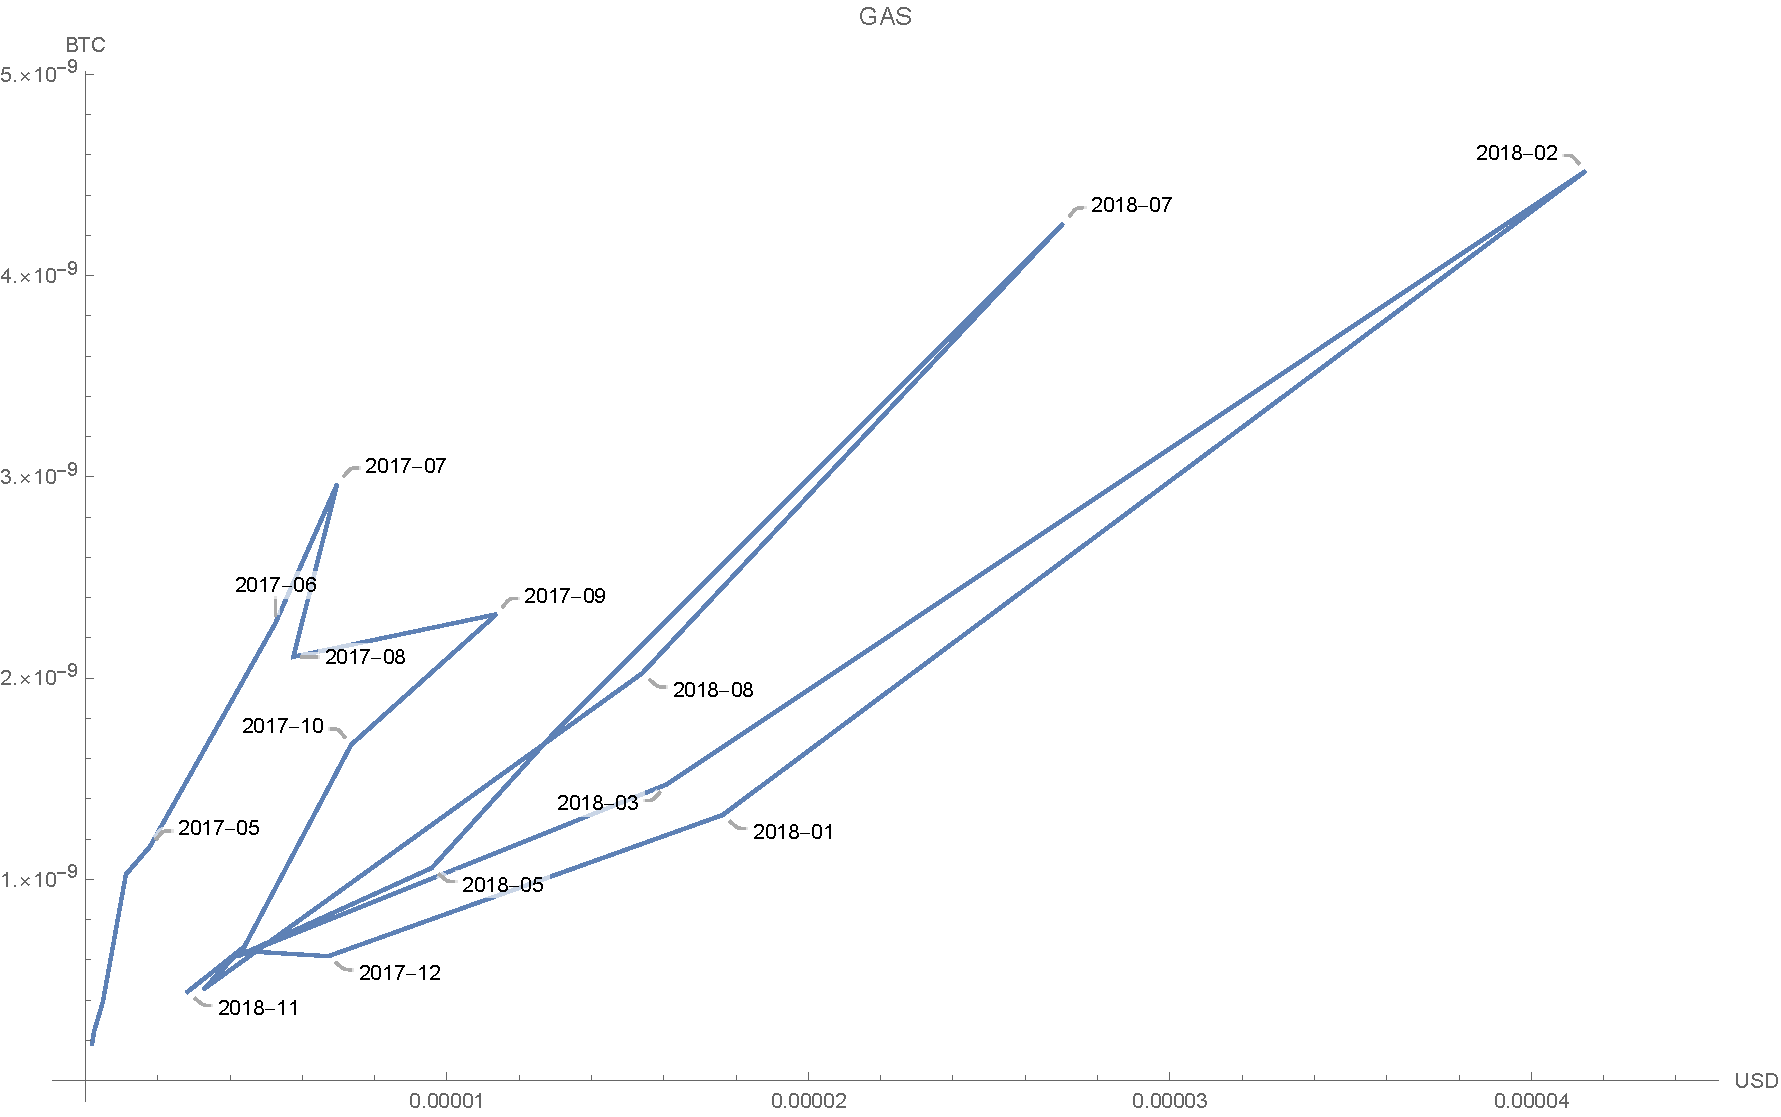
\includegraphics[width=0.95\textwidth]{figures/gas.pdf}
%	\caption{\label{fig:gas} Gas with respect to BTC and gold.}
%\end{figure}
%========================%

%references to figures wrong now!

Figures~\ref{fig:eur}-~\ref{fig:gas} illustrate how the values of EUR, ETH and Gas change with respect to BTC and gold. EUR plot in Figure~\ref{fig:eur} tends to have more movements in the directions 1-5 and 3-7 suggesting that while the value of EUR stays the same according to one axis, it changes according to the other. For instance, between June 2018 and August 2018, the value of EUR increased with respect to BTC, while it stayed the same according to USD. This type of movement suggests that EUR-USD exchange rate is going under less change, whereas BTC-EUR rate is subject to high volatility. On the other hand, in the first half of 2017, while EUR retained its value against BTC, EUR to USD rate went under change.

ETH plot in Figure~\ref{fig:eth} illustrates more volatility against BTC and gold, as there are horizontal, vertical and diagonal changes. The fact that the points are spread in a large range of values indicates drastic changes in ETH price with respect to BTC and Gold.

Compared to Figure~\ref{fig:eur} and Figure~\ref{fig:eth}, gas plot (Figure~\ref{fig:gas}) has mostly diagonal changes, spread over a smaller range. There are less number of changes compared to ETH. Except from the changes between May 2018-July 2018 and January 2018-March 2018, the gas price changes in a smaller range. Even though there are fluctuations in the gas price, it can be inferred that gas price is less volatile than ETH. Also, it worths mentioning that gas is changing over a small scale in x-axis (USD), when compared to Ether's plot over the same axis in a larger interval.


%========================%

\begin{figure}[!htb]
	\centering
	\subfloat[Bitcoin's value with respect to USD and Gold]{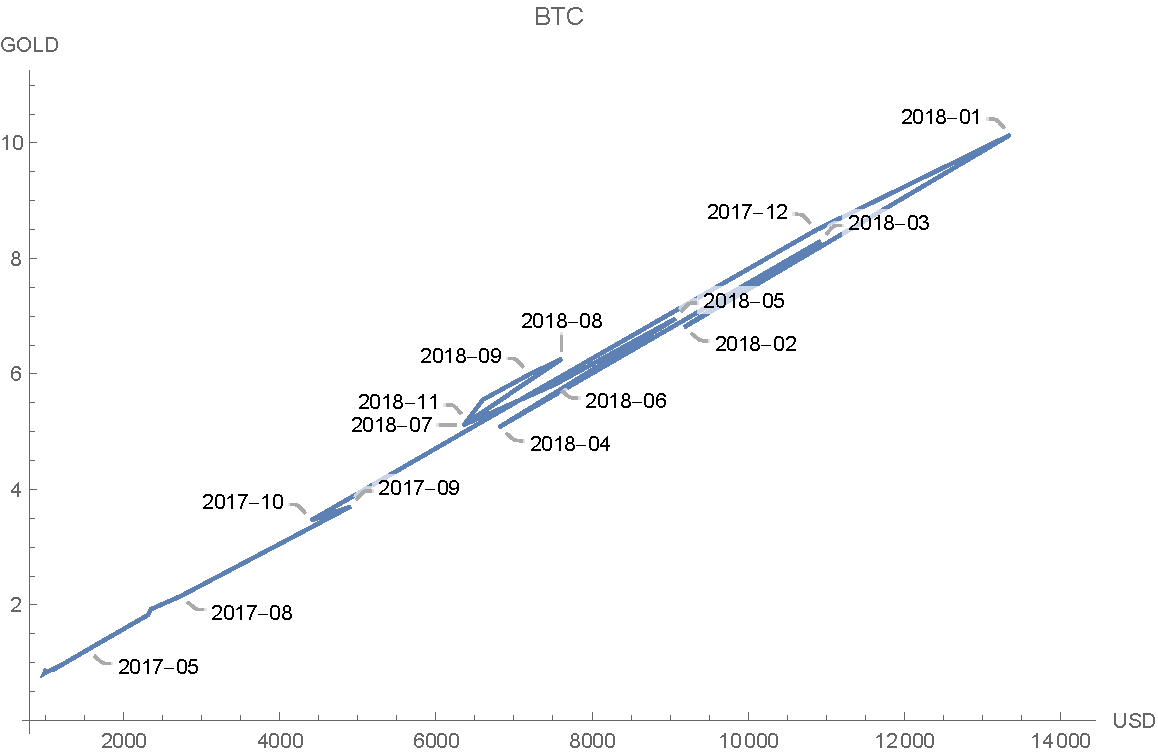
\includegraphics[width=0.75\textwidth]{figures/btc.pdf}\label{fig:btc}}
	\hfill
	\subfloat[Legend]{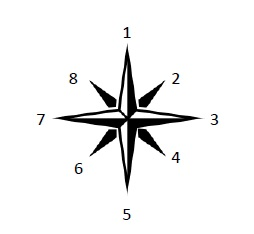
\includegraphics[width=0.25\textwidth]{figures/compass}\label{fig:legend}}
	\caption{BTC}
	\label{fig:Comparison}
\end{figure}
%========================%

\subsection{new graphs}


%========================%

\begin{figure}[!htb]
	\minipage{0.32\textwidth}
	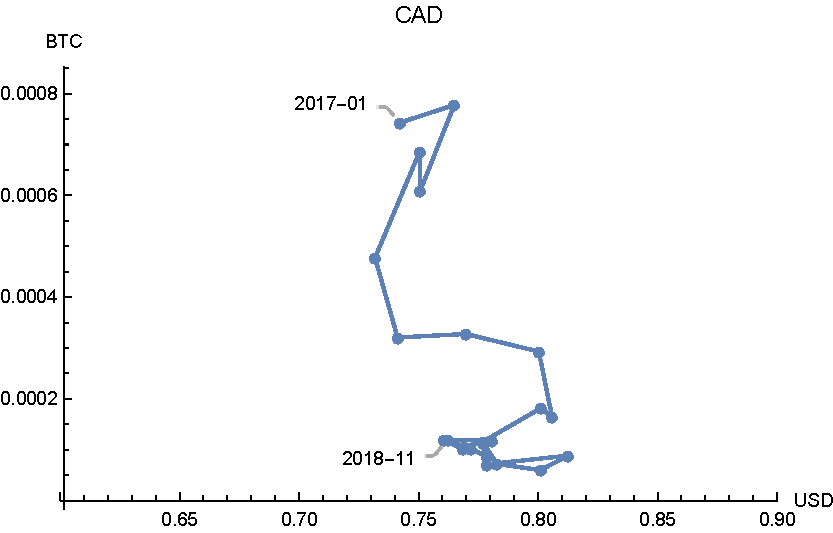
\includegraphics[width=\linewidth]{figures/cad.pdf}
	\caption{CAD with respect to BTC and USD}\label{fig:cad}
	\endminipage\hfill
	\minipage{0.32\textwidth}
	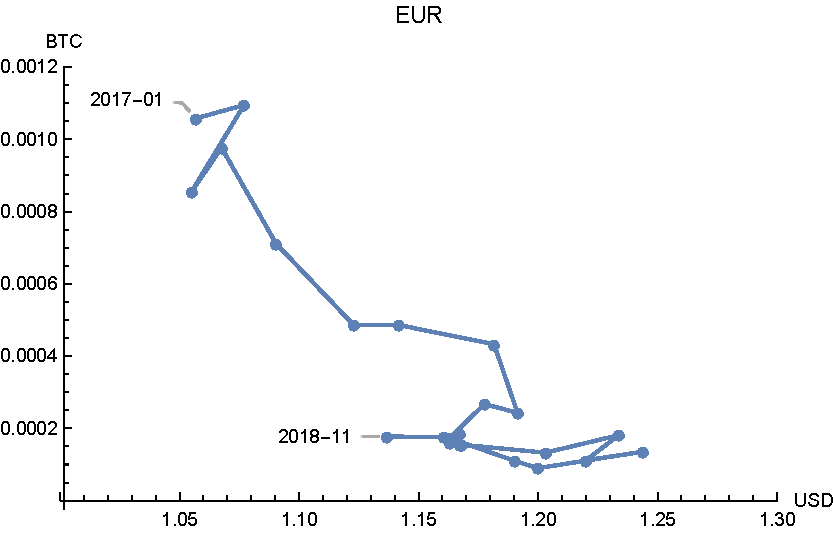
\includegraphics[width=\linewidth]{figures/eur.pdf}
	\caption{EUR with respect to BTC and USD}\label{fig:eur}
	\endminipage\hfill
	\minipage{0.32\textwidth}%
	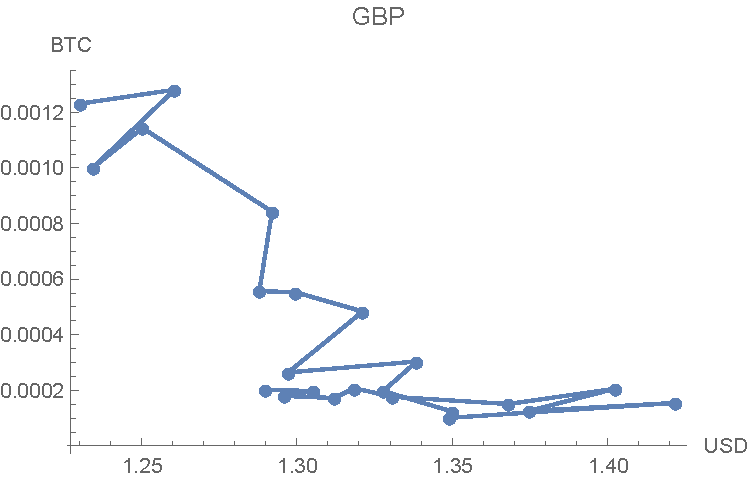
\includegraphics[width=\linewidth]{figures/gbp.pdf}
	\caption{GBP with respect to BTC and USD}\label{fig:gbp}
	\endminipage
\end{figure}
%========================%

\begin{figure}[!htb]
	\minipage{0.32\textwidth}
	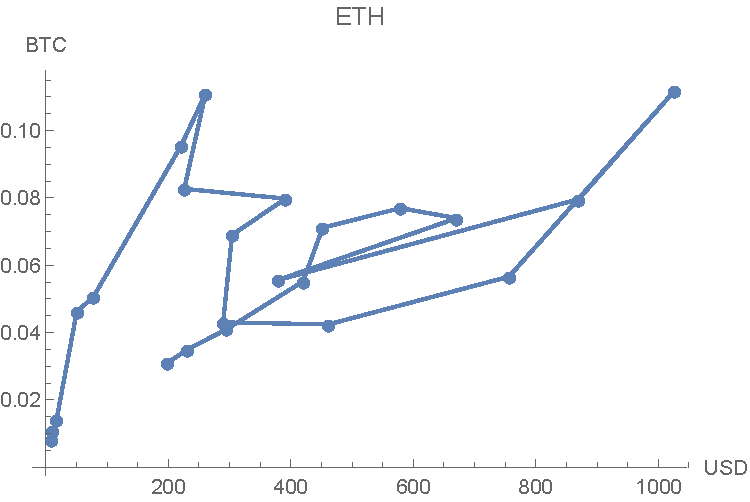
\includegraphics[width=\linewidth]{figures/eth.pdf}
	\caption{ETH with respect to BTC and USD}\label{fig:eth}
	\endminipage\hfill
	\minipage{0.32\textwidth}
	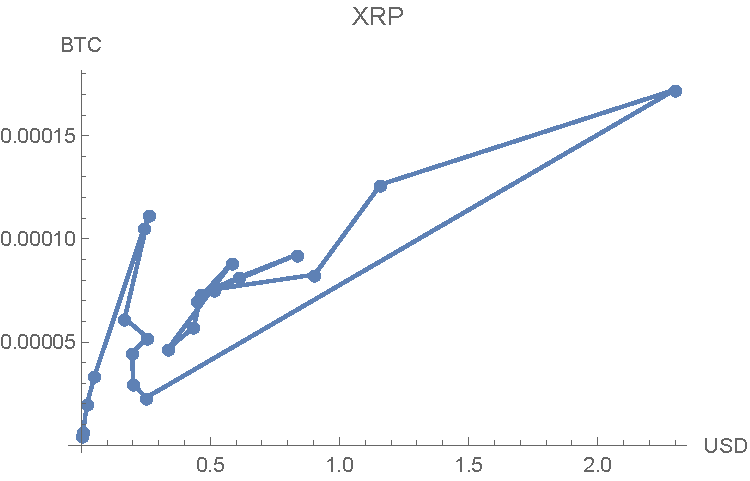
\includegraphics[width=\linewidth]{figures/xrp.pdf}
	\caption{XRP with respect to BTC and USD}\label{fig:xrp}
	\endminipage\hfill
	\minipage{0.32\textwidth}%
	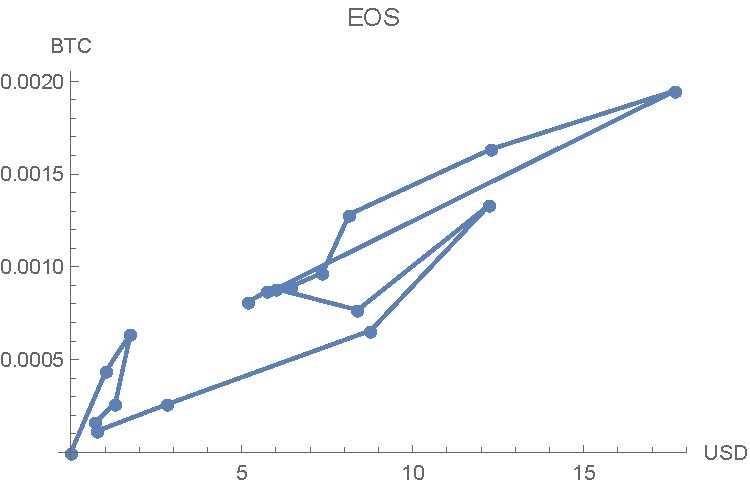
\includegraphics[width=\linewidth]{figures/eos.pdf}
	\caption{EOS with respect to BTC and USD}\label{fig:eos}
	\endminipage
\end{figure}
%========================%

\begin{figure}[!htb]

	\minipage{0.32\textwidth}
	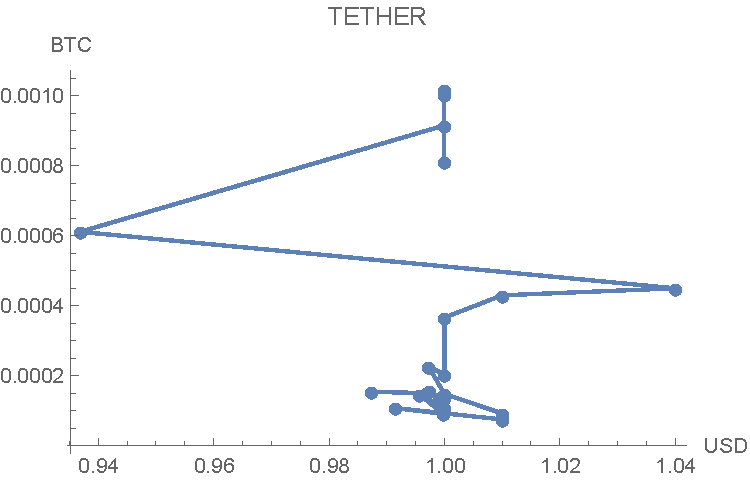
\includegraphics[width=\linewidth]{figures/tether.pdf}
	\caption{Tether with respect to BTC and USD}\label{fig:tether}
	\endminipage\hfill
	\minipage{0.32\textwidth}
	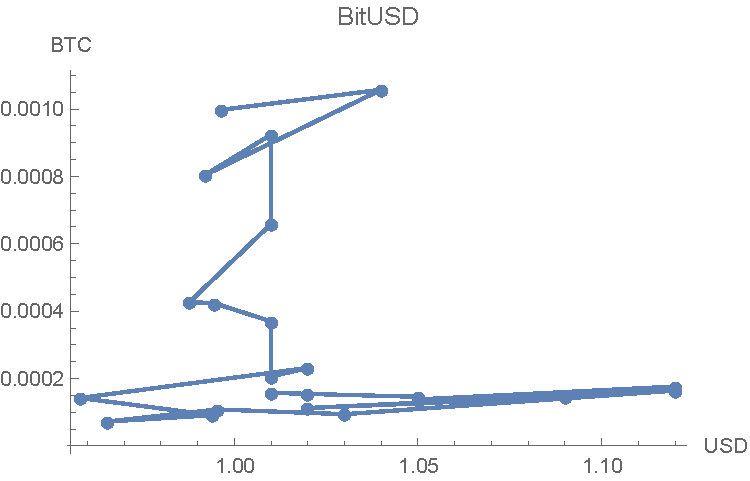
\includegraphics[width=\linewidth]{figures/bitusd.pdf}
	\caption{BitUSD with respect to BTC and US}\label{fig:bitusd}
	\endminipage\hfill
\end{figure}

%========================%

\begin{figure}[!htb]
	\minipage{0.32\textwidth}
	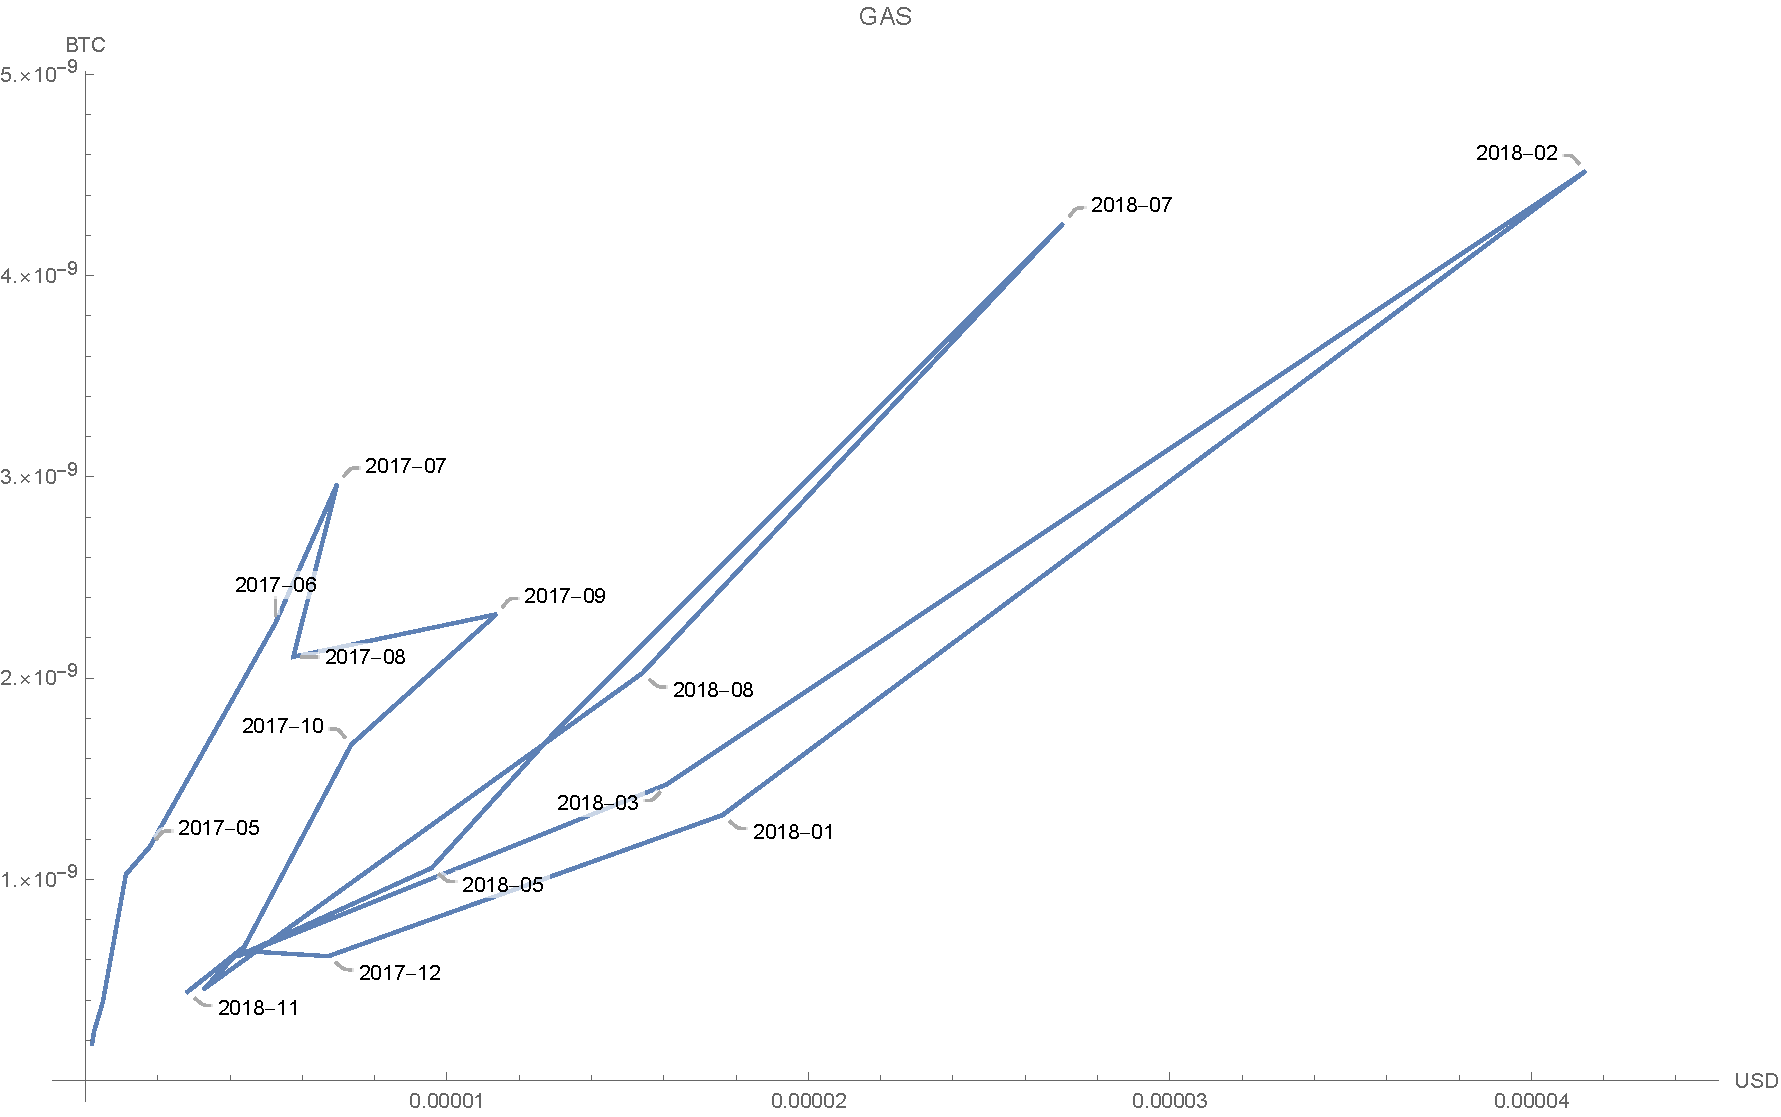
\includegraphics[width=\linewidth]{figures/gas.pdf}
	\caption{Gas with respect to BTC and USD}\label{fig:gas}
	\endminipage\hfill
	\minipage{0.32\textwidth}
	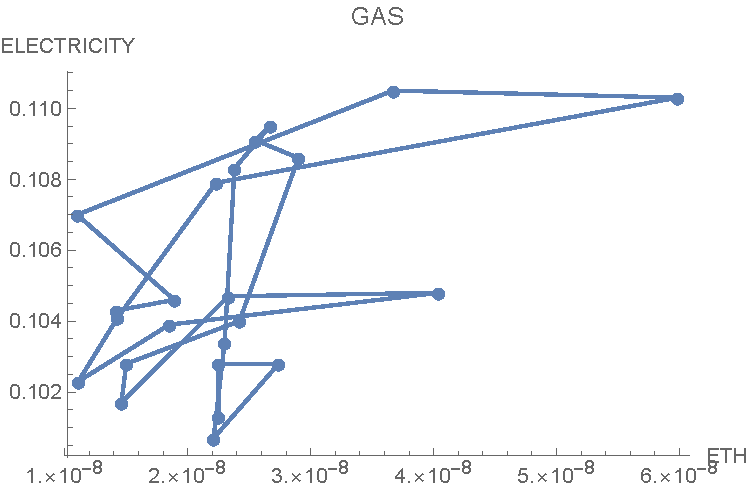
\includegraphics[width=\linewidth]{figures/gasElectricity.pdf}
	\caption{Gas with respect to BTC and USD}\label{fig:gasElectricity}
	\endminipage\hfill
\end{figure}
%==========================================%
%GRAPHS:
%Horizontal: x-axis value is moving
%Vertical: y-axis value is moving
%Diagonal: plot is moving
%About figure1: EUR,CAD and GBP lines are nearly parallel. GBP and EUR come closer after Brexit. Even such an important economical event didn't cause a high volatility compared to BTC price which is more extreme.
%EOS prices between 07-2017 and 11-2018.  01-2017 and  06-2017 price is set to zero
%The rest between 01-2017 and 11-2018
%GBP -(EUR and USD) chart "The pound dropped to its lowest level against the euro in 2017 after Mario Draghi, head of the European Central Bank, pushed the eurozone currency higher by saying he could start tightening monetary policy." September 2017 GBP loses value against both USD end EUR
% CAD,EUR,GBP - (BTC and USD): mostly horizontal movements.
% ETH,EOS,XRP - (BTC and USD): mostly diagonal movements.
% TETHER: Does it artificially inflate BTC price? Do they issue un-backed tokens to reinforce BTC price, then sell BTC to fully back tokens?

%========================%
\begin{figure}[!htb]
	\centering
	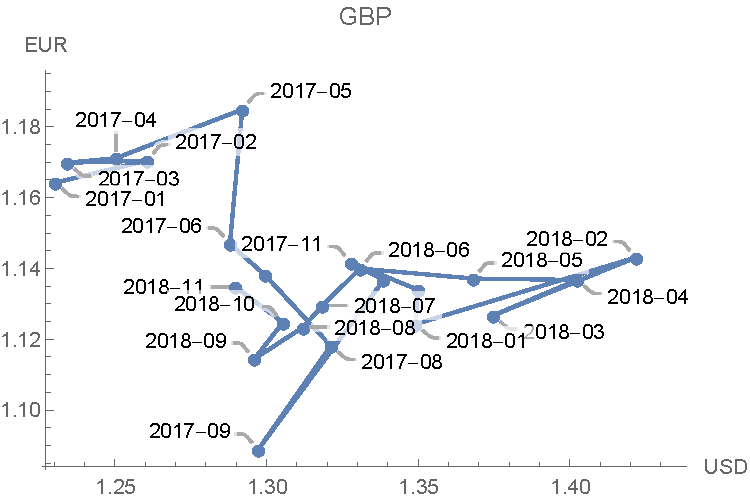
\includegraphics[width=0.75\textwidth]{figures/gbpEURUSD.pdf}
	\caption{\label{fig:gbp1}}
\end{figure}
%========================%
\section{Conclusion and Discussion}
In this paper, we analyze the current state of stablecoins with the various options that have been so far proposed to achieve price stability. We also discuss various issues that stablecoins would address. According to the charts represented in the paper, gas is relatively stable in price, while Bitcoin and Ether show volatile behavior. The reason could be the fact that how users interact with the interface to set the gas price when sending transactions to the Ethereum. By analyzing the properties of gas together with the existing methods to create stablecoin, we can later propose what properties stablecoins should attain.

%==========================================%
\section{The current state of stablecoins (might be needed for the paper)}

%different ways and issues with each. %~\cite{euromoney}
Stablecoins have a market value of \$3 billion and this corresponds to the 1.5\% of the total market value of the cryptoassets~\cite{report}. Each proposing different properties, stablecoins can be categorized into three groups based on the way they achieve stability: fiat-collateralized, crypto-collateralized, and non-collateralized.

~\textbf{1) Fiat-collateralized stablecoins:} These types of stablecoins are backed by fiat currency. Generally, there is a 1:1 peg between the fiat currency and the stablecoin that indicates a convergence between their values~\cite{linkedin}. While USD is currently the most common choice to back the stablecoin, IBM states that they are also interested in projects that use other national fiat currencies, as they will be helpful for their blockchain integration~\cite{cointelegraph}. Tether and TrueUSD are prominent examples of USD pegged tokens.
%Some projects like Digix Gold Token prefer to use gold to back their stablecoin, as gold has a relatively slow increase in its value compared to fiat currencies. %Reference??

~\textit{Discussion about centralization:} In order to back up with stablecoins with fiat, one needs to place trust on a third party. Centralization ensures that the amount of money to back the stablecoin with, is held in an account~\cite{techrev} and the peg is attained. However, involvement of a third party causes controversy, as the third party can deny giving money to the users. Tether explains this point as follows~\cite{cryptoinsider}:

\begin{quote}
``Redemptions will not be unreasonably denied, but we reserve the right to selectively deny redemption and creation of Tethers on a case-by-case basis."
\end{quote}

%Globcoin: less reliance on US dollars but still centralized.~\cite{cryptoinsider}

~\textbf{2) Crypto-collateralized stablecoins:} These types of stablecoins use other cryptocurrencies as a back up value rather than fiat currency. \\ Over-collateralization is needed in this case as the underlying cryptocurrency is also volatile~\cite{linkedin}. MakerDAO and Reserve use this approach -- utilizing a smart contract to back the stablecoin with another cryptocurrency~\cite{cointelegraph}.

If there is a black swan event~\footnote{A black swan event is characterized as being unexpected, random and having significant effects to the current situation. This type of an event is hard to predict~\cite{swan}.} where the underlying currency loses its value and does not worth anything, the stablecoin also loses its value~\cite{coinsexplained}.  Due to the over-collateralization in this type of stablecoins, the loss of value will be drastic. This is the reason that a group of experts strongly discourage this approach.

~\textbf{3) Non-collateralized stablecoins:} Unlike the previous types, this group of stablecoins are not backed by fiat currencies or another cryptocurrency. Here, the stability is achieved algorithmically which helps to provide better scalability~\cite{report}.

Basis is one of the first projects of this type that achieves price stability using the dual-token model~\cite{cryptoinsider}. In this method, there is dynamic adjustment of the existing supply of the stablecoin. While one token is stable, the other is used to achieve the stability of the value. If the value of Basis increases (an increase over \$1), more Basis tokens are produced to increase the supply which will lead to a decrease in the price and if there is a decrease in the price, a bond that is worth a Basis token is issued and some Basis tokens are bought to decrease the supply~\cite{euromoney}.


\section{Issues that stablecoins address}
As mentioned in Section~\ref{Intro}, currencies have to serve as a store of value, a unit of account, and a medium of exchange~\cite{smithin2002money}. To do so, they have to denote a minimum level of value stability. In this regard, stablecoins are proposed to fulfill these properties, due to their non-fluctuating value compared to fiat currencies or any other alternative\eg commodity. In addition, they purport to solve a group of critical issues that were introduced by cryptocurrencies. In this section, we discuss these issues.

\subsection{Cryptocurrencies as Medium of Exchange}
Despite the fast growth of the cryptocurrencies and decentral applications, there is still little deployment of them in the daily payment procedures of businesses. The main reason is that these assets are volatile in the price and hence highly risky to be deployed by merchants and retailers \ie it is impossible for a company employer to provide the employees' incomes in a volatile cryptocurrency \eg BTC that has a high level of future value and price uncertainty. On the other hand, having a stable price over the time, stablecoins can serve as a true medium of exchange, while they preserve all the advantages of using cryptocurrencies as opposed to fiat currencies.

\subsection{Cryptocurrencies as Unit of Account}
Money has to serve also as a unit of account-- the common measure that sets price to goods and services. Fiat currencies \eg USD, EUR \etc serve this functionality correctly, so they are used as units of account in the US and Europe respectively. Unfortunately, cryptocurrencies such as BTC, not having a stable price, do not seem to be used as a unit of account, hence will not be able to serve as money. However, given the price stability that stablecoins offer, they have a higher chance to be used as a digital representation of a unit of account.

\subsection{Cryptocurrencies as Store of Value}
Any asset, commodity, or money that maintains its value is called a store of value. As mentioned in Section~\ref{Intro}, highly volatile cryptocurrencies (\ie Bitcoin) cannot fulfill this property of money, as they cannot maintain their purchasing value for long-term. In contrast, stablecoins can be accepted as a store of value as their price remains stable over the time.

\subsection{Lending with Cryptocurrencies}
Despite quite a few blockchain applications in financial technologies, there has been little deployment of lending.
Lending is difficult to be deployed on the blockchains, bdue to the monetary instability observed in the existing cryptocurrencies~\cite{okoyetoward}. This volatility has led the cryptocurrencies to be used more as speculative investments instead of serving as store of value and unit of account. In a lending situation with volatile currencies, where their values are being depreciated or appreciated over time, the cash taker will eventually owe more than what he has borrowed or the vice versa. Therefore, the volatility in the value of cryptocurrencies causes serious concerns and difficulties both for cash takers and cash providers~\cite{okoyetoward}. In contrast, lending perfectly works if a loan is done with a stable cryptocurrency, whose value remains stable over the time.

\subsection{Remittance}

Although cryptocurrencies, especially Bitcoin, play a revolutionary role in financial systems, they are yet not easy to transact with due to their volatile characteristics. Therefore with stablecoins, one can benefit from decentralized nature of the token, while there is no price volatility risk. In addition, stablecoins make the cross border payments, remittances, easier.



\section{January 9 Meeting notes}
\begin{itemize}
	\item discussion about the price of a coin backed by fiat currency:
	what happens to the value of token if half of the supply disappears?
	what if everyone wants to sell their tokens and get the CAD, USD etc equivalent?
	why would you want to sell the tokens?: not a successful currency then
	\item BTC: nothing backs it, not unit of account, good medium of exchange
	\item Gold: not unit of account, not medium of exchange
	\item why do we overload the function of money? (no need to fulfill all three properties)
	\item IMF's SDR (Special Drawing Rights) only Unit of account?
	\item The model of backing a currency works? Why, why not?
	\item Discussion about BTC and the hydrocost
	\item Controlling the amount of money in the circulation: government bonds
	\item What is stability?
	Who decides?
	What do you change?
	What parameters to consider to apply the change?
	\item In the case of BTC, cryptocurrencies the number of transactions, how old the coin is affects the value?
	\item Can a method to stabilize a currency be gamed?: is this method economically sound?
	\item Bank of England: whitepapers
	\item Coindesk: list of stablecoins mentioned.
\end{itemize}

\subsection {Discussion on the notes}
\begin{itemize}
\item What if sob steals all of the reserve (CAD)? then there are two scenarios: 1) people know the reserve is gone so they start converting their tokens back to CAD (for example) so the price of the token will drop. 2) people do not know that the reserve is gone and nobody goes to bank to exchange his token, in this case, it does not affect the price but at the end the token goes bankrupt.
What if only half of the reserves disappears? nobody goes to the bank to ask for CAD and  it doesn’t change anything, like USD and gold.

\item Q: We may want to ask this from ourselves when writing the paper: should we actually design a currency (meet 3 properties)

\item supply and demand :government makes people use their currency

\item BTC and Hydro are not directly connected (not pegging) BTC is not backed by anything

\item  as soon a sth price goes more that 1 dollar > you sell people tokens for 1 dollar so that the price stays the same (currency boards) : pegging : it works until you have your reserves.
In Canada: they control the amount of money in circulation, increase decrease the supply of money, how they increase the supply of money now? whom do they give it? Answer: they buy things (open market operations)- they go out and buy governments bonds, they borrow the money, from whom? they announce it public so in 5 years they pay you + 5\% (IOU) \par
They’re doing this based on some information they get, to stabilize the economics but based on what? first it was based on the exchange rate of the CAD (failed) now they are looking at interest rate: there is a certain interest rate they look for, the interest rate where banks lend money to other banks

\item central bank tried to stabilizes the economy based on exchange rate but it failed.
\item in BTC :
\begin {itemize}
\item what nub are you turning? (coinbase for now but there could be more)
\item who will turn the nub? A: a  person B: algorithm that blockchain decides BUT how blockchain knows based on what they could turn the nub (third questions)
\item what are you looking at to know when to turn the nub? number of tx in block, liquidity in money
\end{itemize}

\textbf{TO DO:}
search query on coindesk and we found these projects that are mostly used : looking for the project name \textbf{(Coindesk : every article mentioning stable coin until January 11, 2019)}
find a report that says how central bank stabilize : bank of England has a bunch of white papers -> "Banks used the exchange rate but it failed “ phrase is from one of it white papers.

\end{itemize}


